Systèmes, entités, variables, événements, processus… 
% TODO: upload diagramme de classe

Le système est composé de deux partie : un programme, écrit en Java,  qui implémente la boucle de simulation, et un ficher Excel qui contient les données issues du programme est qui les traite pour en ressortir des résultats statistiques.
\\
Le programme Java implémente une boucle de simulation évènementiel telle que décrite par la figure~\ref{replique}. 
Le processus d'initialisation remplit un agenda qui contient les évènements d'arrivés d'avion dans l'espace aérien de l'aéroport, ainsi que les instants de changement de météo.



 \begin{figure}[h]
   \caption{\label{replique} Boucle de simulation}
 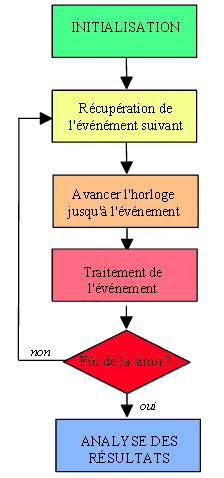
\includegraphics{replique_simu.bmp}
 \end{figure}






\begin{figure}[h]
   \caption{\label{class_diagramm} Diagramme de classe}
 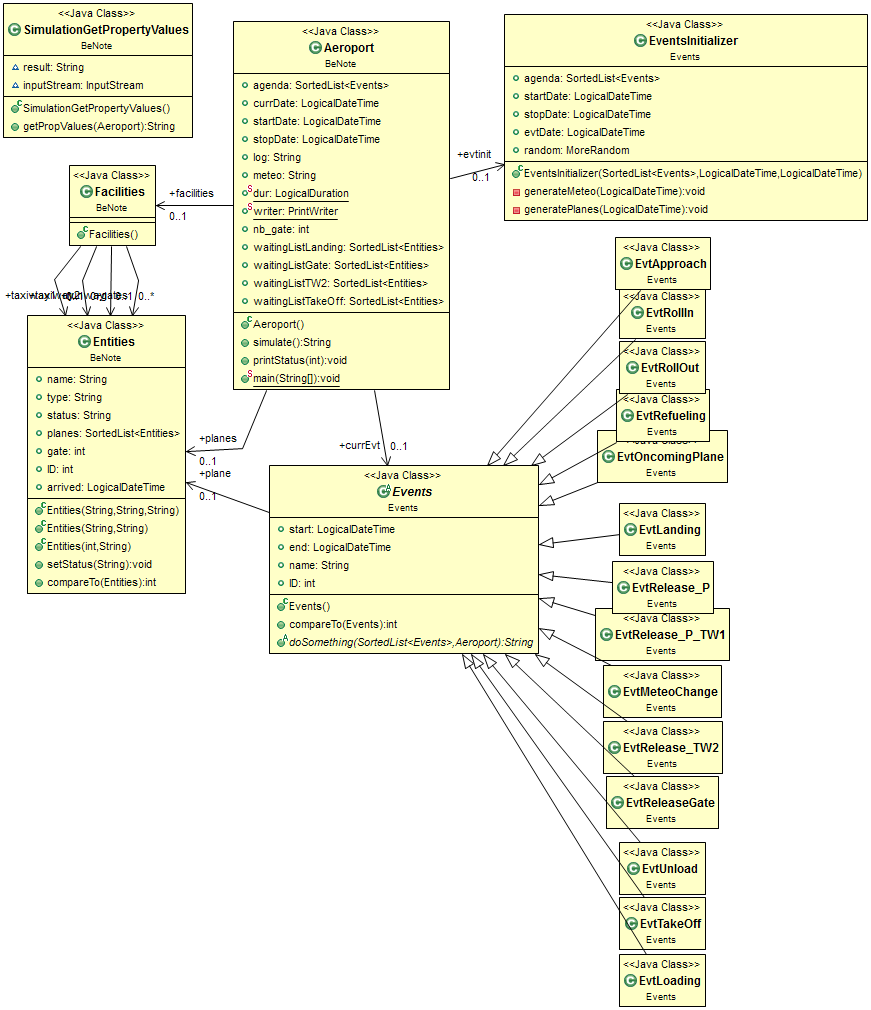
\includegraphics{Class_Diagramm.png}
 \end{figure}
 
